\chapter{Problematyka zagadnienia}
\label{ch:problematyka}

%---------------------------------------------------------------------------
\section{Charakterystyka choroby Parkinsona}
\label{sec:charakterystykaPD}

Choroba Parkinsona (PD) to zwyrodnieniowe schorzenie mózgu, które wiąże się z objawami ruchowymi, takimi jak spowolnienie ruchowe,
drżenie, sztywność oraz zaburzenia chodu i równowagi.
Ponadto, to schorzenie może prowadzić do różnorodnych powikłań niemotorycznych, obejmujących zaburzenia poznawcze, stany psychiczne,
trudności ze snem oraz dolegliwości sensoryczne, w tym ból.
Początkowe objawy często rozwijają się stopniowo, nasilając się w miarę upływu czasu.
Postęp choroby prowadzi do znacznego stopnia niepełnosprawności, co może wymagać wsparcia i opieki.
U wielu osób zdiagnozowanych z chorobą Parkinsona występują także zmiany w sferze psychicznej i behawioralnej, takie jak
trudności ze snem, depresja, problemy z pamięcią oraz uczucie przewlekłego zmęczenia.

\begin{figure}[htbp]
	\centering
	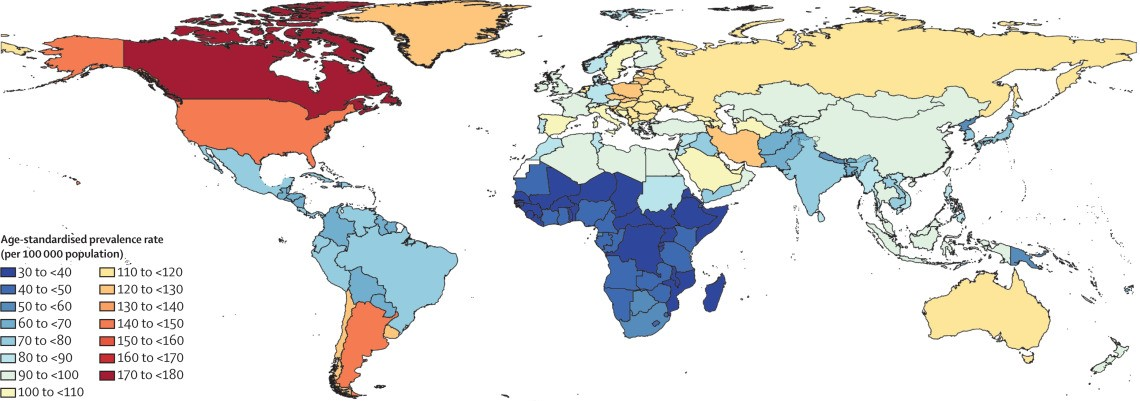
\includegraphics[width=0.9\textwidth]{./img/map}
	\caption{Choroba Parkinsona na świecie \cite{global_PD}}
    \label{fig:PD_map}
\end{figure}

Zgodnie z danymi przedstawionymi w raporcie Światowej Organizacji Zdrowia \cite{WHO}, choroba Parkinsona (PD) stanowi obecnie narastający problem na skalę światową. Zarówno wskaźniki niepełnosprawności, jak i zgony związane z tą chorobą rosną szybciej niż w przypadku innych zaburzeń neurologicznych.

W ciągu ostatnich 25 lat zaobserwowano podwojenie częstości występowania PD na całym świecie.
Globalne szacunki na rok 2019 wskazują, że liczba osób cierpiących na PD przekroczyła 8,5 miliona.
Co więcej, analizy obrazują, że w 2019 roku PD spowodowała aż 5,8 miliona lat życia z niepełnosprawnością, co oznacza wzrost o 81\% w porównaniu z danymi z roku 2000.
Jednocześnie liczba zgonów związanych z tą chorobą wyniosła 329 000, co stanowi wzrost o ponad 100\% w porównaniu z rokiem 2000 \cite{global_PD}.

PD jest istotną sprawą dotyczącą zdrowia publicznego, ponieważ jej częstotliwość występowania związana jest ze zjawiskiem starzejącego się społeczeństwa.
Razem z innymi chorobami neurodegeneracyjnymi, takimi jak choroba Alzheimera, PD ma szanse stać się drugą zaraz za nowotorami przyczyną zgonów do 20240 roku (WHO).

W Polsce z chorobą Parkinsona zmaga się około 100 tys. pacjentów, z czego około 20\% jest już w stadium zaawansowanym
według informacji przekazywanych przez Fundację Chorób Mózgu.
Ponadto co roku w naszym kraju wykrywanych jest ok. 8 tys. nowych zachorowań.
Nowe zachorowania nadal skorelowane są z wiekiem, średnia wieku chorych wynosi 60 lat, niestety wzrasta odsetek chorych wśród osób młodych (nawet w wieku 20 lat).

Przyczyna PD nie jest znana, ale uważa się, że powstaje w wyniku złożonej interakcji pomiędzy czynnikami genetycznymi i
narażeniem na czynniki środowiskowe, takie jak pestycydy, rozpuszczalniki i zanieczyszczenia powietrza.
Niektóre przypadki PD wydają się być dziedziczne, a kilka przypadków można przypisać określonym wariantom genetycznym.
Chociaż uważa się, że genetyka odgrywa rolę w chorobie Parkinsona, w większości przypadków choroba nie występuje rodzinnie \cite{National_Institute_on_Aging_2022}.

\begin{figure}[htbp]
	\centering
	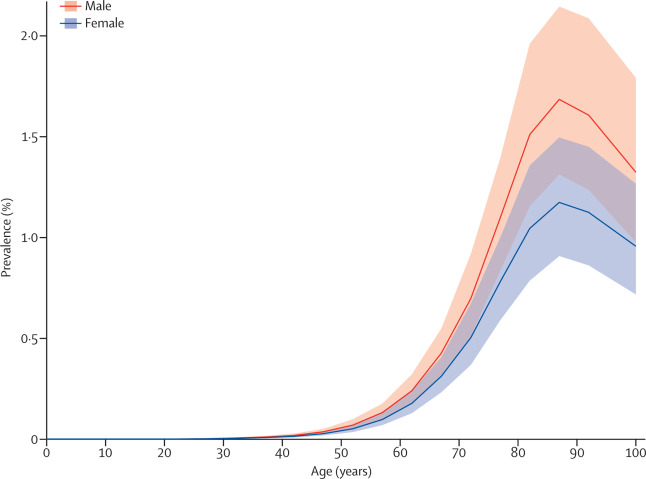
\includegraphics[width=0.6\textwidth]{./img/PD_prevalence}
	\caption{Rozpowszechnienie choroby Parkinsona w zależności od wieku \cite{global_PD}}
    \label{fig:PD_prevalance}
\end{figure}

Chociaż każdy może być narażony na ryzyko rozwoju choroby Parkinsona to obserwuje się, że choroba Parkinsona występuje częściej u mężczyzn niż u kobiet,
a wiek stanowi kluczowy element wpływający na ryzyko zachorowania, co można zobaczyć na Rys.\ref{fig:PD_prevalance}.
Statystyki pokazują, że ryzyko zachorowania rośnie wraz z wiekiem, chociaż choroba może dotyczyć także młodszych osób.
U większości osób z PD po raz pierwszy choroba rozwija się po 60 roku życia, około 5\% do 10\% doświadcza jej początku przed 50 rokiem życia.
Postacie choroby Parkinsona o wczesnym początku są często, choć nie zawsze, dziedziczne i niektóre formy zostały powiązane z
określonymi zmianami w genach \cite{National_Institute_on_Aging_2022}.

%---------------------------------------------------------------------------

\subsection{Objawy choroby}
\label{subsec:objawy}

Najbardziej widoczne oznaki i objawy choroby Parkinsona pojawiają się, gdy komórki nerwowe w zwojach podstawy mózgu,
obszarze mózgu kontrolującym ruch, ulegają uszkodzeniu i/lub obumierają.
Zwykle te komórki nerwowe lub neurony wytwarzają dopaminę.
Kiedy neurony obumierają lub ulegają uszkodzeniu, wytwarzają mniej dopaminy, co powoduje problemy z poruszaniem się
związane z chorobą.
Na ten moment nie wiadomo co powoduje śmierć neuronów.
Zanikają również zakończenia nerwowe, które wytwarzają norepinefrynę, główny przekaźnik chemiczny
współczulnego układu nerwowego, który kontroluje wiele funkcji organizmu, takich jak tętno i ciśnienie krwi.
Utrata norepinefryny może pomóc wyjaśnić niektóre cechy choroby Parkinsona związane z brakiem ruchu, takie jak zmęczenie,
nieregularne ciśnienie krwi, zmniejszony ruch pokarmu w przewodzie pokarmowym i nagły spadek ciśnienia krwi, gdy osoba wstaje z pozycji siedzącej lub leżącej.

\vspace{0.5cm}
Do czterech głównych objawów choroby Parkinsona zalicza się:
\begin{itemize}[itemsep=0.05pt]
	\item drżenie rąk, ramion, nóg, szczęki lub głowy,
	\item sztywność mięśni, gdy mięśnie pozostają skurczone przez długi czas,
	\item powolność ruchu,
	\item zaburzenia równowagi i koordynacji, czasami prowadzące do upadków.
\end{itemize}

\vspace{0.15cm}
Pozostałe objawy mogą obejmować:
\begin{itemize}[itemsep=0.05pt]
	\item depresja i inne zmiany emocjonalne,
	\item trudności w połykaniu, żuciu i mówieniu,
	\item problemy z układem moczowym lub zaparcia,
	\item problemy skórne.
\end{itemize}


Objawy choroby Parkinsona oraz tempo jej postępu mogą znacząco różnić się wśród poszczególnych osób.
Na wczesnym etapie choroby objawy są subtelne i kształtują się stopniowo.
Często zaczynają się od jednej strony ciała lub nawet jednej kończyny.
W miarę jak choroba rozwija się, dotyka ona ostatecznie obu stron, jednak niekiedy objawy mogą być bardziej intensywne po jednej stronie niż po drugiej.
Niektórzy pacjenci z chorobą Parkinsona doświadczają pewnych zwiastunów przed wystąpieniem charakterystycznych cech, takich jak sztywność czy drżenie.
Mogą to być trudności ze snem, problemy z wypróżnianiem, utrata węchu czy także zespół niespokojnych nóg.
Warto jednak zaznaczyć, że niektóre z wymienionych objawów mogą również występować w procesie naturalnego starzenia się \cite{National_Institute_on_Aging_2022}.


Chociaż tempo postępu choroby Parkinsona zazwyczaj jest powolne, w końcu ma to wpływ na codzienne funkcjonowanie osoby dotkniętej tą dolegliwością.
Wykonywanie zwykłych czynności, takich jak praca, prowadzenie domu czy uczestnictwo w spotkaniach towarzyskich z przyjaciółmi, może stawać się wyzwaniem.

%---------------------------------------------------------------------------

\subsection{Terapia osób chorych}
\label{subsec:terapia}
Obecnie brak jest kuracji na chorobę Parkinsona, dlatego terapia skupia się na przywracaniu pacjentom zdolności funkcjonowania
lub, w przypadkach zaawansowanych, na poprawie jakości życia.
Zgodnie z aktualnym standardem medycznym, w terapii wykorzystuje się różnorodne metody, w tym leczenie farmakologiczne, głęboką stymulację mózgu oraz rehabilitację \cite{National_Institute_on_Aging_2022}.

Leczenie farmakologiczne choroby Parkinsona opiera się na zwiększeniu poziomu dopaminy w mózgu, co wpływa na kontrolę objawów
ruchowych i niezwiązanych z ruchem. Główną terapią jest lewodopa, która jest przetwarzana przez komórki nerwowe w dopaminę.
Leczenie lewodopą często łączy się z karbidopą, która zmniejsza skutki uboczne i ilość potrzebnej lewodopy.
Stosuje się też inne terapie farmakologiczne o różnych zasadach działania m.in. pobudzające produkcję dopaminy,
zwiększające ilość dopaminy poprzez spowolnienie jej rozkładu, redukujące ruchy mimowolne czy zmniejszające drżenie i sztywność mięśni.

W przypadku pacjentów, u których leczenie farmakologiczne nie przynosi oczekiwanych efektów, może być rozważana Głęboka Stymulacja Mózgu (ang. \emph{Deep Brain Stimulation} - DBS).
W tym procederze chirurgicznym lekarz implantuje elektrody w określone obszary mózgu, łącząc je z małym urządzeniem elektrycznym umieszczonym w klatce piersiowej.
Poprzez bezbolesne stymulowanie konkretnych obszarów mózgu kontrolujących ruch, DBS może pomóc w zmniejszeniu wielu objawów związanych z ruchem,
takich jak drżenie, spowolnienie ruchu i sztywność.

Kluczową rolę w leczeniu odgrywa rehabilitacja neurologiczna, rozpoczynając się już od momentu postawienia diagnozy.
Jej wsparcie jest nieocenione w łagodzeniu zaburzeń chodu, głosu, drżenia, sztywności oraz pogorszenia funkcji umysłowych.
Wśród różnorodnych terapii, znajdują się między innymi:
\begin{itemize}[itemsep=0.1pt]
	\item zbilansowana dieta: wspiera ogólne samopoczucie pacjenta,
	\item ćwiczenia fizyczne: wzmacniają mięśnie, poprawiają równowagę, elastyczność i koordynację,
	\item masaż terapeutyczny: pomaga w redukcji napięcia mięśniowego oraz przynosi ulgę w objawach,
	\item joga i tai chi: wspomagają rozciąganie i elastyczność ciała, wpływając korzystanie na zdolność ruchową,
	\item rehabilitacja foniczna: pomaga w eliminowaniu trudności w mówieniu,
	\item psychoterapia: zapewnia wsparcie i umożliwia pacjentom pełne cieszenie się życiem pomimo choroby.
\end{itemize}

Rehabilitacja neurologiczna stanowi nieodzowny element kompleksowego podejścia do zarządzania chorobą Parkinsona, pomagając pacjentom w utrzymaniu jak najwyższej jakości życia.

%---------------------------------------------------------------------------

\section{Metody diagnozowania i monitorowania}
\label{subsec:diagnostyka}

Diagnostyką choroby Parkinsona zajmują się neurolodzy i geriatrzy.
Jej rozwój jest długotrwały, a w początkowych latach klinicznie niemal niewidoczny, co utrudnia wczesne rozpoznanie.
Subtelne objawy często są uważane za skutek starzenia się lub błędnie diagnozowane jako inne zaburzenia neurologiczne.
Kluczowym elementem w tym stadium jest dokładny wywiad, badanie fizykalne oraz identyfikacja objawów przez lekarza.
Następnie diagnoza jest rozwijana poprzez badania laboratoryjne  oraz obrazowe.
Niestety, wyniki tych badań rzadko potwierdzają diagnozę od razu.

Początkowo pacjent zwykle konsultuje się z lekarzem pierwszego kontaktu, który powinien dokonać wstępnej diagnozy i skierować do neurologa.
W tej fazie diagnozy przeprowadza się szczegółowy wywiad, uwzględniający rodzaj, nasilenie oraz okres występowania objawów, a także
obecność chorób neurozwyrodnieniowych w rodzinie.
Neurolog przeprowadza kompleksowe badanie neurologiczne, identyfikując symptomy takie jak sztywność mięśni, ograniczenia w
ruchu (spowolnienie, trudności w poruszaniu się), drżenia spoczynkowe (np. w głowie, palcach rąk) oraz zaburzenia postawy i równowagi
(zgarbienie, niestabilność, upadki). Kolejne badania są wykonywane w celu potwierdzenia lub wykluczenia diagnozy \cite{diagnostyka_Sitek, Loscalzo_2022}.

\renewcommand{\labelenumi}{\alph{enumi})}
\begin{enumerate}
	\item Badania laboratoryjne
	\item[] Obecnie brak specyficznych badań laboratoryjnych krwi, które potwierdzałyby diagnozę choroby Parkinsona.
Niemniej jednak, takie badania są użyteczne w wykluczaniu innych chorób o podobnym przebiegu.
Wykonuje się podstawowe badania, takie jak morfologia krwi, elektrolity, poziom glukozy, TSH, próby wątrobowe, mocznik, kreatynina oraz poziom witaminy B12.

	\item Badania obrazowe
	\item[] Badania obrazowe głowy są przeprowadzane w celu wykluczenia innych chorób o podobnych objawach.
Pomimo że nie są one szczególnie pomocne w diagnozowaniu choroby Parkinsona, odgrywają ważną rolę w diagnostyce różnicowej.
Do tych badań zalicza się tomografię komputerową, ultrasonografię mózgu (USG) oraz rezonans magnetyczny głowy (MRI). Chociaż badania te nie potwierdzają choroby Parkinsona, mogą ujawnić obecność guzów mózgu czy wodogłowia.
Międzynarodowe kryteria rozpoznania choroby Parkinsona nie nakładają obowiązku wykonywania badań obrazowych w celu potwierdzenia diagnozy.
Warto jednak wiedzieć, że dostępne są również zaawansowane techniki obrazowania, takie jak PET (pozytonowa emisyjna tomografia) oraz SPECT (tomografia emisyjna pojedynczego fotonu),które pozwalają na obserwację metabolizmu w układzie pozapiramidowym. Skan DAT (skan transportera dopaminy) jest przykładem SPECT i może być sugerowany przez specjalistę.
Mimo to, ostateczna diagnoza opiera się na objawach oraz wynikach badania neurologicznego. Większość pacjentów nie wymaga skanowania DAT.

	\item Test z lewodopą
	\item[]Test polega na podaniu pacjentowi podejrzewanemu o chorobę Parkinsona preparatu z lewodopą.
Jeśli następuje poprawa po zażyciu, istnieje wysokie prawdopodobieństwo, że pacjent rzeczywiście cierpi na chorobę Parkinsona.
W przypadku braku poprawy, konieczne może być dalsze rozszerzenie diagnostyki.

	\item Badania genetyczne
	\item[] Choroba Parkinsona może występować w rodzinach, co skłania do rozważenia diagnostyki genetycznej u pacjenta i jego krewnych.
Badania te są wskazane, gdy lekarz podejrzewa dziedziczne występowanie choroby.
Obecnie zidentyfikowano 12 mutacji genów, które mogą wpływać na ryzyko zachorowania na chorobę Parkinsona.
Należy jednak zaznaczyć, że badania genetyczne są kosztowne.
Proszę, daj znać, czy taka wersja Ci odpowiada, czy może potrzebujesz dalszych zmian.


	\item Badania węchu
	\item[] Większość osób z chorobą Parkinsona (90\%) doświadcza zaburzeń węchu, manifestujących się hiposomią (osłabienie węchu), także we wczesnym stadium choroby.
Jednak nie obserwuje się tych zaburzeń w przypadku zaniku wieloukładowego i postępującego porażenia nadjądrowego.

	\item Badania neuropsychologiczne i neuropsychiatryczne
	\item[] Badania te służą identyfikacji zaburzeń poznawczych i emocjonalnych u osób z podejrzeniem choroby Parkinsona.
Psycholodzy i psychiatrzy mają za zadanie diagnozować łagodne zaburzenia poznawcze, otępienie, a także zaburzenia psychotyczne, lękowe, zachowania, kontroli impulsów i depresję.
Proces diagnostyczny jest dostosowany indywidualnie do możliwości pacjenta.
\end{enumerate}

Naukowcy badają test amplifikacji nasion alfa-synukleiny, zdolny do wykrywania choroby Parkinsona przed pojawieniem się objawów.
Test identyfikuje skupiska białka alfa-synukleiny w płynie rdzeniowym, charakterystyczne dla ciał Lewy'ego w mózgu.
Badanie z 2023 roku na ponad 1000 osobach wykazało, że test trafnie rozpoznał chorobę Parkinsona w 87,7\% przypadków.
Wyniki sugerują, że ten test może zmienić podejście do diagnozy, badań i terapii choroby Parkinsona.
Planuje się przyszłe badania oraz nadzieję na mniej inwazyjne metody, takie jak próbki krwi, do przeprowadzania testu \cite{Mayo_Clinic_PD}.

Objawy przypominające chorobę Parkinsona mogą być spowodowane różnymi zaburzeniami, takimi jak zanik wieloukładowy, demencja z ciałami Lewy'ego czy postępujące porażenie nadjądrowe. Te schorzenia są z kolei diagnozowane jako parkinsonizm.

Właściwe odróżnienie między tymi chorobami jest istotne, ponieważ leczenie i podejście terapeutyczne różnią się \cite{National_Institute_on_Aging_2022}.
Badania medyczne oraz reakcja na leczenie farmakologiczne mogą pomóc w ustaleniu dokładnej przyczyny.
Ważne jest, aby uzyskać szybką i dokładną diagnozę.

Choroby o podobnym przebiegu do choroby Parkinsona obejmują m.in. postępujące porażenie nadjądrowe, zanik wieloukładowy, drżenie samoistne, choroby naczyniowe mózgu, otępienie, reumatyzm oraz inne \cite{diagnostyka_Sitek}.
Różnicowanie tych schorzeń jest kluczowe dla właściwego leczenia i zarządzania pacjentem.

Diagnostyka różnicowa choroby Parkinsona obejmuje różne formy parkinsonizmu oraz inne stany neurodegeneracyjne.
Chociaż ostateczną diagnozę można ustalić tylko na podstawie badania mózgu po zgonie, wcześniej zdefiniowane kryteria diagnostyczne pozwalają na dokonanie diagnozy klinicznej.
Przyjęcie ram czasowych (3-10 lat) dla postawienia klinicznie potwierdzonej diagnozy choroby Parkinsona opiera się na empirycznych dowodach.
Wnioski płynące z badania \cite{ROSSI202153} sugerują, że diagnoza klinicznie potwierdzonej choroby Parkinsona może zabierać od kilku miesięcy do kilku lat, zależnie od indywidualnych czynników oraz reakcji na terapię lewodopą.

Chorobę Parkinsona wykluczają także pewne kryteria.
Zalicza się do nich historię wielokrotnych urazów głowy, przebyte zapalenie mózgu, podobne objawy u więcej niż jednej osoby w rodzinie,
leczenie neuroleptykami w momencie objawów, przebyte udary mózgu z nasilonymi objawami parkinsonowskimi, długotrwałe ustąpienie objawów oraz objawy po jednej stronie ciała przy chorobie trwającej ponad 3 lata.

Pomocnym narzędziem w dianostyce są szeroko stosowane skale oceny choroby Parkinsona.
Stanowią istotne narzędzie w monitorowaniu stanu pacjentów oraz ocenie postępów choroby.
Te strukturalne i skwantyfikowane metody pomagają lekarzom i opiekunom ocenić stopień nasilenia objawów ruchowych,
jak również wpływ choroby na codzienne funkcjonowanie pacjenta.
Popularne skale, takie jak Skala Hoehn-Yahra, Skala UPDRS (Unified Parkinson's Disease Rating Scale) oraz Skala Schwab-England,
umożliwiają obiektywną analizę symptomów i wsparcie w podejmowaniu decyzji terapeutycznych.
Dzięki tym narzędziom możliwe jest dostosowanie leczenia do indywidualnych potrzeb pacjenta oraz śledzenie skuteczności terapii na przestrzeni czasu.


Proces diagnozowania choroby Parkinsona to zadanie wymagające czasu i precyzji.
W celu skutecznej identyfikacji i monitorowania pacjentów z tym schorzeniem, zaleca się regularne wizyty kontrolne u neurologów specjalizujących się w zaburzeniach ruchowych. Tego rodzaju wizyty pozwalają na bieżące ocenianie stanu zdrowia oraz objawów, umożliwiając dokładną diagnozę choroby Parkinsona.

Obecnie proces diagnozy jest wyjątkowo złożony i wieloetapowy.
W odpowiedzi na te wyzwania, naukowcy koncentrują się na opracowaniu bardziej efektywnych narzędzi diagnostycznych.
Poszukiwane są innowacyjne metody, które przyspieszą i usprawnią ten proces.
Rozwinięcie skuteczniejszych narzędzi diagnostycznych przyniesie korzyści nie tylko finansowe, ale także pozwoli na szybsze i trafniejsze udzielanie pomocy pacjentom cierpiącym na chorobę Parkinsona.
Poprawa diagnozy pomoże podnieść standard życia osób dotkniętych tym schorzeniem, co jest priorytetem dla społeczności medycznej i pacjentów.

W nadchodzących latach, dążenie do wypracowania bardziej efektywnych metod diagnozowania choroby Parkinsona będzie kluczowym krokiem w zapewnieniu lepszej opieki zdrowotnej i poprawie jakości życia pacjentów.

%---------------------------------------------------------------------------
%---------------------------------------------------------------------------

\section{Znaczenie głosu}
\label{sec:znaczenie_glosu}
Choroba Parkinsona, będąca rezultatem zaburzonej funkcji układu nerwowego, wywołuje różnorodne objawy w różnych obszarach ciała.
To złożone zjawisko stanowi istotny temat badań dla wielu naukowców na całym świecie.
Badania nad analizą mowy stanowią obszar szczególnego zainteresowania.
W przypadku choroby Parkinsona objawy zaburzeń mowy zwykle stają się widoczne w średniozaawansowanym stadium schorzenia, co oznacza, że przez długi okres mowa pozostaje relatywnie nienaruszona.
Rozpoznanie tych zaburzeń może być niekiedy trudne, gdyż wymaga odróżnienia, czy powstały one na skutek samej choroby, czy też są rezultatem naturalnego
procesu starzenia się organizmu.

Proces starzenia wpływa na fizjologiczne osłabienie słuchu, co z kolei może prowadzić do zmian w brzmieniu głosu.
Głos staje się osłabiony, wykazujący tendencję do drżenia, a także jego zakres tonacji może ulec zawężeniu.

Objawy zaburzeń mowy i głosu związane z chorobą Parkinsona nie są łatwo dostrzegalne dla osób bez specjalistycznej wiedzy w tej dziedzinie.
Przeważnie zdolność rozumienia mowy pozostaje niezmieniona.
Niemniej jednak, w trakcie spontanicznych wypowiedzi pacjenci zaczynają ograniczać ilość przekazywanych informacji i mogą napotykać trudności w składaniu
pełnych zdań.
Te trudności nie wynikają koniecznie z ubytku słownictwa, ale raczej z nieprawidłowego doboru słów.
Wskazujące na podłoże chorobowe objawy obejmują między innymi \cite{Szurek_2018, Kuryłowicz_2019}:
\begin{itemize}[itemsep=0.1pt]
	\item pogłębione wyciszenie głosu,
	\item mowę powolną, monotonną i przerywaną,
	\item zubożenie mimiki,
	\item nadmierne ślinienie się,
	\item niewyraźną i zamazaną artykulację,
	\item skrócony czas fonacji
	\item chuchający i tremolujący głos
	\item spłaszczoną barwę i obniżone natężenie
	\item niewłaściwą koordynację mięśni nasady, które mogą być zwiotczałe lub zbyt napięte,
	\item czasami przyspieszenie tempa wypowiedzi w jej końcowej fazie, co może utrudnić zrozumienie pacjenta.
\end{itemize}

Te objawy pojawiają się w średniozaawansowanym stadium choroby, są wystarczająco wyraźne, aby mogły zostać zauważone słuchowo przez specjalistów.
Niemniej jednak badania wskazują, że istnieją subtelne zmiany w głosie, które pojawiają się jeszcze wcześniej, w fazie przedobjawowej \cite{2023_PD_voice}.

W roku 2000 przeprowadzono badanie akustyczne i percepcyjne cech głosu pacjentów z chorobą Parkinsona, zależnie od stopnia nasilenia choroby \cite{https://doi.org/10.1080/136828200410654}.
W nagraniach głosowych, składających się z przedłużonej samogłoski /a/, śpiewu gamy oraz 1-minutowego monologu, stwierdzono, że głosy pacjentów z PD,
zarówno we wczesnych, jak i późniejszych stadiach choroby, charakteryzowały się ograniczoną percepcyjnie zmiennością tonu i głośności, chropowatością
oraz zmniejszoną głośnością.

Wspomniane badanie sugerowało również, że głosy pacjentów z PD wykazywały nadmierne drganie, wysoką częstotliwość podstawową (szczególnie u mężczyzn) oraz zmniejszoną zmienność częstotliwości podstawowej (szczególnie u kobiet).
Część z tych cech głosu nie wydawała się pogarszać w miarę postępu choroby, jednak cechy takie jak oddech, monotonność i jednolitość mowy, niska głośność oraz ograniczony maksymalny zakres częstotliwości fonacyjnej były bardziej zauważalne w późniejszych stadiach choroby Parkinsona.

Podobne badanie przeprowadzone przez Gamboę i innych (1997) wykazało, że w porównaniu z grupą kontrolną, pacjenci z PD wykazywali wyższy jitter, niższy stosunek harmonicznych do szumów (H/N), mniejszą zmienność częstotliwości i intensywności mowy, niższy zakres fonacyjny oraz wyższą częstotliwość obecności głosu o niskim natężeniu, jednotonowość i zatrzymanie głosu.
Wskazano również, że te cechy nie wykazywały znaczącego związku z czasem trwania choroby \cite{GAMBOA1997314}.

\vspace{0.5cm}

Mnogość objawów, które są zauważalne w głosie, motywuje do uzwględnienia ich w diagnostyce.
Prowadzone są badania, które wykorzystują analizę mowy do wykrywania patologii i schorzeń związanych z narządem głosu, takich jak ostre zapalenie krtani czy porażenie nerwu krtaniowego wstecznego.
Może to w przyszłości pozwolić na identyfikację problemów zdrowotnych, na przykład wśród osób pracujących głosem, jak nauczyciele, bez konieczności inwazyjnych badań gardła.
Podobne podejście można zastosować do diagnozowania i monitorowania chorób neurodegeneracyjnych.
Badania naukowe wskazują, że analiza głosu może stanowić podstawę dla automatycznej diagnostyki oraz monitorowania choroby Parkinsona.

Takie podejście niesie za sobą wiele korzyści, które mogą rewolucjonizować sposób diagnozowania oraz monitorowania tej neurodegeneracyjnej choroby:

\renewcommand{\labelenumi}{\alph{enumi})}
\begin{enumerate}
	\item \textbf{unikalność i wieloaspektowość analizy głosu}
	\item[] W kontekście diagnostyki choroby Parkinsona, analiza głosu prezentuje się jako innowacyjne rozwiązanie, skupiające się na aspekcie mowy i jakości głosu pacjenta. Głos, będący wskaźnikiem stanu układu nerwowego oraz zdolności komunikacyjnych, oferuje szeroką gamę informacji, które mogą być kluczowe dla procesu diagnozowania. Różnorodność parametrów akustycznych i fonacyjnych, które można zbadać i przeanalizować, otwiera drzwi do kompleksowej oceny zmian zachodzących w organizmie pacjenta.
	\item \textbf{szybka wykrywalność subtelnych zmian}
	\item[] Wczesne objawy choroby Parkinsona często bywają trudne do dostrzeżenia, szczególnie w standardowych badaniach klinicznych. Jednym z głównych wyzwań jest wykrycie tych subtelnych zmian w ich wczesnym stadium. Analiza głosu pozwala na szybką identyfikację takich subtelności, które mogą pojawić się we wczesnych fazach choroby. Taka wczesna detekcja otwiera drzwi do natychmiastowej interwencji terapeutycznej, zanim objawy nabiorą większej intensywności, co potencjalnie może wpłynąć na spowolnienie progresji choroby i poprawę jakości życia pacjenta.
	\item \textbf{wsparcie dla specjalistów i pacjentów oraz ocena stanu pacjenta}
	\item[] Wprowadzenie analizy głosu jako narzędzia diagnostycznego dostarcza specjalistom nowych perspektyw w obszarze choroby Parkinsona. Logopedzi, foniatrzy i lekarze mogą korzystać z obiektywnych danych akustycznych do dokładnej oceny zmian w mowie i jakości głosu pacjenta. Dodatkowo, analiza taka może być wykorzystana do oceny stanu pacjenta oraz sugerowania odpowiednich interwencji, włączając zmiany w leczeniu farmakologicznym. To pozwala na dostosowanie terapii w oparciu o konkretne i mierzalne parametry głosu, co może prowadzić do lepszych rezultatów leczniczych.
	Z drugiej strony, pacjenci otrzymują bardziej konkretną ocenę swojego stanu oraz lepiej dostosowane terapie, co przyczynia się do zwiększenia efektywności procesu leczenia. Analiza głosu, jako narzędzie obiektywne, może stanowić podstawę do podejmowania decyzji terapeutycznych, opartych na konkretnej ocenie zmian w mowie i głosie pacjenta. W ten sposób pacjenci otrzymują dostosowane i zoptymalizowane interwencje, co może przyczynić się do szybszej poprawy ich stanu zdrowia.
	\item \textbf{szybkość i bezwględność}
	\item []Analiza głosu, jako nieinwazyjne badanie, przyczynia się do skrócenia czasu wymaganego na ocenę pacjenta. Badanie to jest szybkie, wygodne i bezpieczne, co może zachęcać pacjentów do systematycznego uczestnictwa w procesie diagnostycznym. Szczególnie istotne jest to w przypadku pacjentów, którzy mogą mieć ograniczoną zdolność do przemieszczania się. Ponadto, jako narzędzie obiektywne, analiza głosu eliminuje subiektywne oceny, co przekłada się na większą pewność diagnostyczną i lepsze prowadzenie terapii.
	\item \textbf{nowe horyzonty diagnostyczne}
	\item[] Zastosowanie analizy głosu w diagnostyce choroby Parkinsona otwiera drzwi ku nowym, zaawansowanym metodologiom diagnozowania i leczenia, które mogą mieć znaczący wpływ na poprawę jakości życia pacjentów. Dzięki zaawansowanym technologiom, takim jak sztuczna inteligencja i uczenie maszynowe, możliwe jest jeszcze dokładniejsze ocenienie parametrów głosu oraz ich interpretacja w kontekście choroby. Taka innowacyjna metoda ma potencjał stania się szybkim, nieinwazyjnym wsparciem diagnostycznym i terapeutycznym, przyczyniając się do polepszenia opieki nad pacjentami dotkniętymi chorobą Parkinsona.
\end{enumerate}

Analiza głosu jako narzędzie diagnostyczne przy chorobie Parkinsona otwiera drzwi ku nowym, zaawansowanym metodologiom diagnozowania i leczenia, które mogą mieć znaczący wpływ na poprawę jakości życia pacjentów.

Dodatkowo, analiza taka może być wykorzystana do oceny stanu pacjenta oraz sugerowania odpowiednich interwencji, włączając zmiany w leczeniu farmakologicznym.
W konsekwencji, taka innowacyjna metoda ma potencjał stania się szybkim, nieinwazyjnym wsparciem diagnostycznym i terapeutycznym, przyczyniając się do polepszenia
opieki nad pacjentami dotkniętymi chorobą Parkinsona.